\chapter{Konzeption}
Im Folgenden wird ein Konzept für die Implementierung des Tools vorgestellt, das  die Ziele der Bachelorarbeit erfüllen soll.
\section{Traversierung aller relevanten Dateien} 
Softwareprojekte bestehen aus Hunderten von Dateien, die nicht alle Quellcode enthalten. Beispielsweise gehören Konfigurationsdateien, Ressourcedateien wie Bilder oder binäre Dateien zu den Dateien, bei denen eine Analyse der Softwaredokumentation im Hinblick auf die begrenzte Zeit für die Bachelorarbeit nicht implementierbar ist. Daher ist es sinnvoll, bestimmte Dateien bei der Analyse auszuschließen beziehungsweise nur bestimmte Dateien zu betrachten. Bei einer Weiterentwicklung des Tools nach Abschluss der Bachelorarbeit kann das Tool auf andere Dateitypen ausgeweitet werden, um so ein besseres Gesamtbild über die Softwaredokumentation zu erhalten.

Um die relevanten Dateien zu finden, wird zunächst ein übergeordnetes Verzeichnis benötigt, was bei Softwareprojekten aber der Standard sein sollte. Dieses Verzeichnis kann dann rekursiv durchlaufen werden und somit die Liste aller darin gespeicherten Dateien abgerufen werden. Die relevanten Dateien können dann durch Überprüfung ihres Dateinamens mittels bestimmter Regeln ermittelt werden, die der Benutzer des Tools festlegen kann.

Beim JavadocEvaluator wird hierzu die NPM-Bibliothek Minimatch \footnote{\href{https://github.com/isaacs/minimatch}{Minimatch GitHub-Repository (besucht am 07.01.2022)}} verwendet, die es ermöglicht, Dateinamen mit Wildcard-Patterns zu vergleichen. Zum Beispiel könnte der Dateiname \enquote{test.txt} mit der Wildcard \enquote{test.*} verglichen werden und die Bibliothek würde eine Übereinstimmung melden.

\section{Parsing der Java-Dateien} 
Jede Datei, die relevant sein soll, muss anschließend weiterverarbeitet werden. Für die Bewertung der Dokumentation sind nur wenige Bestandteile relevant. Beispielsweise sind alle For-Schleifen, If-Verzweigungen und viele andere Komponenten in Methodenrümpfen nicht relevant, da diese nur mit normalen Kommentaren und nicht mit Javadoc kommentiert werden; (sie werden dennoch unstrukturiert als Zeichenkette gespeichert, damit Metriken diese Information eventuell nutzen können). Aus diesem Grund müssen die notwendigen Informationen extrahiert werden. Zudem ist es ein Ziel der Arbeit , eine Erweiterbarkeit auf andere objektorientierte Programmiersprachen zu ermöglichen. Daher müssen die Informationen in ein abstraktes Format gebracht werden, welches eine gute Annäherung für die meisten objektorientierten Programmiersprachen ist. Beispielsweise unterscheiden sich die Zugriffsmodifizierer vieler Programmiersprache, sodass eine einheitliche Schnittstelle schwer umsetzbar ist. Daher enthält die abstrakte Repräsentation nur Informationen, ob eine Komponente als öffentlich markiert ist. Dies ist sinnvoll, da öffentliche Komponenten als Teil der öffentlichen Schnittstelle eher dokumentiert werden sollten als nicht öffentliche und eine weitergehende Differenzierung kaum Vorteile bietet. In einigen Programmiersprachen wie z. B. Python gibt es keine expliziten öffentliche Komponenten, jedoch existieren de facto Standards für Bezeichner, sodass beispielsweise private Komponenten zwei Unterstriche als Präfix haben.

Außerdem werden in der abstrakten Repräsentation die Vererbung etwas vereinfacht dargestellt, indem nicht zwischen Basisklassen und Schnittstellen unterschieden wird, da es auch hier Unterschiede zwischen Programmiersprachen gibt, und die Informationen über die Vererbung, falls sie überhaupt von einer Metrik verwendet wird, vermutlich nicht so detailreich sein müsste. Zudem werden Konstruktoren als Methoden mit den Namen \enquote{constructor} und Schnittstellen als Klassen repräsentiert, da auch hier eine zu feine Spezifikation nicht notwendig sein wird.  

  

In anderen Fällen gibt es jedoch viele Gemeinsamkeiten zwischen objektorientierten Programmiersprachen; so gibt es in  allen relevanten Sprachen Klassen, Methoden und Felder, die alle einen Namen haben. Des Weiteren haben Methoden und Felder einen (Rückgabe-)Type und Methoden besitzen Parameter, die ihrerseits durch einen Namen und einen Typen definiert sind. Einige Sprachen sind zwar nicht stark typisiert, jedoch kann für nicht bekannte Datentypen ein Alias wie \enquote{Any} oder  \enquote{Object} verwendet werden.  Zudem sind viele Komponenten hierarchisch; in den meisten Sprachen können beispielsweise Klassen andere Klassen enthalten, sodass diese abstrakte Struktur diese Tatsache berücksichtigen müsste. 

Um dennoch sprachspezifische Funktionen anbieten zu können, besitzt jede Komponente ein Feld mit dem Typen \textit{ComponentMetaInformation}, das wie oben erwähnt die Information enthält, ob eine Komponente als öffentlich angesehen werden soll. Dieser Typ, welches eine Schnittstelle ist, kann von einer Klasse implementiert werden, um Parser für andere Programmiersprachen die Möglichkeit zu geben, zusätzliche sprachspezifische Informationen zu speichern. Beim Java-Parser wird diese Funktion beispielsweise genutzt, um zu speichern welche \enquote{checked} Ausnahmen eine Methode werfen kann, sodass später ein Vergleich mit der Javadoc möglich ist. Die Schnittstelle enthält nur die Anforderung, eine \textit{isPublic}-Methode anzubieten und kann daher für viele andere objektorientierte Programmiersprache Informationen speichern, die für einige Metriken eventuell nützlich sind. 

Abbildung \ref{fig:uml_parsing} gibt einen Überblick über die Klassen, die im Arbeitspaket \enquote{Parsing} verwendet wurden.
\begin{figure}
    \centering
    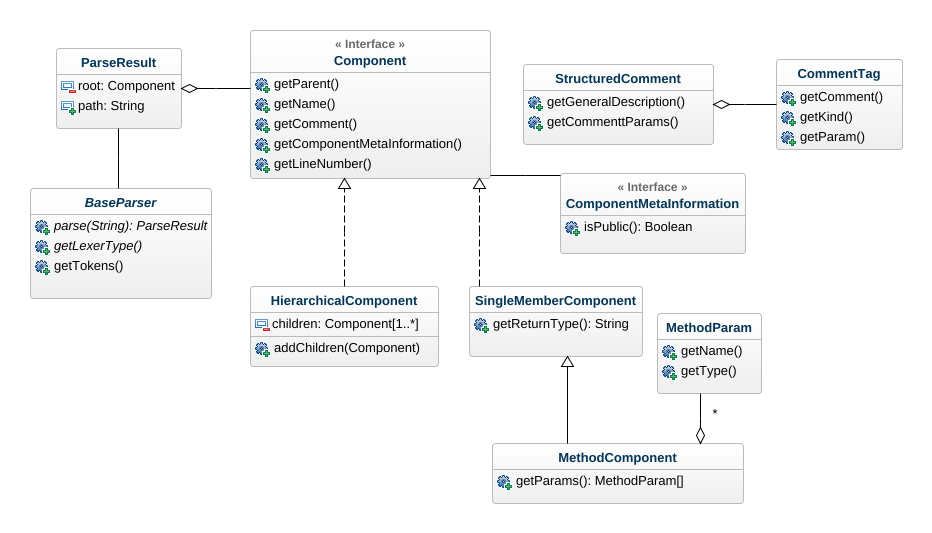
\includegraphics[width=\columnwidth]{figures/uml/parsing.png}
    \caption{UML-Diagramm mit allen wichtigen Klassen für das Parsen}
    \label{fig:uml_parsing}
\end{figure}
\section{ANTLR4}
Um die Java-Dateien zu parsen, wird die Bibliothek ANTLR4\footnote{\href{https://www.antlr.org/}{ANTLR Website (besucht 07.01.2022)}} verwendet, die kostenlos verfügbar ist. Diese Bibliothek kann nicht nur viele Programmiersprachen, sondern auch selbst geschriebene Sprachen parsen, sofern eine passende Grammatik verfügbar ist. Daneben gibt es noch Bibliotheken wie Bison, PEG.JS, die ebenfalls eine ähnliche Aufgabe erfüllen können. Allerdings gibt es bereits vordefinierte Grammatiken für ANTLR4, sodass ein erheblicher Aufwand gespart werden konnte.  

Eine andere Möglichkeit zum Parsen der Java-Dateien ist die NPM-Bibliothek \enquote{java-parser} \footnote{\href{https://www.npmjs.com/package/java-parser}{Java-Parser (besucht 07.01.2022)}}. Dies hätte den Vorteil, dass das Parsen, welches nicht der Hauptfokus dieser Bachelorarbeit ist, ausgelagert wird und so Fehler vermieden werden. Allerdings kann diese Bibliothek nicht die Verbindung zwischen einer Komponente und der dazugehörigen Javadoc herstellen, sodass eine Benutzung dieser Bibliothek die Arbeit deutlich erschwert hätte. Daher fiel die Wahl auf \textit{ANTLR4}. Außerdem besteht die Möglichkeit, eine eigene Grammatik für Java zu schreiben, da die originale Grammatik für Java sämtliche Kommentare ignoriert. Da dies jedoch deutlich komplizierter war als erwartet, wurde dennoch entschieden, die von vielen Entwicklern geschriebene Grammatik zu verwenden (siehe Kapitel \ref{chapter:antlr4_impl}).

\section{Lexer und Parser}
Eine Grammatik für Programmiersprachen besteht immer aus einer Lexer-Grammatik und eine Parser-Grammatik, die jeweils vom Lexer bzw. Parser in dieser Reihenfolge verarbeitet werden, um so eine Baumstruktur einer Quellcodedatei zu erhalten. Der Lexer erstellt aus einer Quellcodedatei eine Liste von Tokens. Dabei ist ein Token eine Gruppierung von einem oder mehreren Zeichen, die eine weitergehende Bedeutung haben. Beispielsweise können Schlüsselwörter einer Programmiersprache oder Operatoren als Token klassifiziert werden. Diese Tokens sind grundsätzlich kontextunabhängig, das heißt für die gleiche Zeichenkette wird das gleiche Token verwendet. Jeder Token wird durch seine Zeichenkette und den Tokentyp klassifiziert

Listing \ref{lst:lexer_example} zeigt zur Verdeutlichung der Syntax eine Zeile aus der Lexer-Grammatik. 
		\begin{figure} [htbp]
			\lstinputlisting
			[caption={Beispielhafte Syntax vom Lexer},
			label={lst:lexer_example},
			captionpos=b, basicstyle=\footnotesize, tabsize=2, showstringspaces=false,  numbers=left]
			{figures/lexer_example.g4}
		\end{figure}

Eine Zeile in der Lexer-Grammatik beginnt mit den Namen eines Tokens, gefolgt von einem Doppelpunkt und dann einem regulären Ausdruck, der dieses Token beschreibt. In der beispielhaften Lexer-Grammatik wird ein Javadoc-Kommentar definiert, das mit \enquote{/**} beginnt, dann folgen beliebige Zeichen und endet mit \enquote{*/}. Per Konvention haben die Bezeichner der Tokens nur Großbuchstaben, sie müssen auf jeden Fall mit einem Großbuchstaben beginnen \cite[S. 3]{ANTLR:APredicated-<i>LLk</i>ParserGenerator}. 

Der nächste Schritt ist das  Parsen. Dabei werden die im vorherigen Schritt generierten Tokens, die als Liste vorliegen, genommen und in eine hierarchische Baumstruktur umgewandelt, wobei hier der Kontext die entscheidende Rolle spielt. ANTLR4 lädt ein Token nach dem anderen und prüft ob es, basierend auf der aktuellen Position in der Baumstruktur, eine Regel gibt, die durch diesen Token erfüllt wird. Wenn es mehrere mögliche Pfade gibt, lädt ANTLR4 so viele Tokens bis die nächste Regel eindeutig feststeht. Gibt es dennoch Uneindeutigkeiten, so wird die Regel genommen, die als erstes in der Parser-Datei geschrieben wurde.\cite[S. 10ff.]{TheDefinitiveANTLR4Reference}

So kann eine vereinfachte Parser-Grammatik für Java einen Baumknoten definieren, der eine generelle Methode beschreibt. Eine Methode besteht aus Rückgabetyp, Bezeichner und Parameterliste. Die Parameterliste kann dann als eine Liste von Datentyp-Bezeichner-Paare aufgelöst werden. Der Rückgabetyp einer Methode ist allerdings anders zu verstehen als der Datentyp eines Parameters, da jeder Datentyp eines Parameters auch ein gültiger Rückgabetyp ist, was jedoch nicht umgekehrt der Fall ist; so ist \textit{}{void} ein gültiger Rückgabetyp, aber kein Datentyp. Listing \ref{lst:parser_example} zeigt einen typischen Ausschnitt aus einer Parser-Grammatik, wobei zur Übersichtlichkeit nicht alle Regeln und Tokens aufgelistet sind:
		\begin{figure} [htbp]
			\lstinputlisting
			[caption={Beispielhafte Syntax vom Parser},
			label={lst:parser_example},
			captionpos=b, basicstyle=\footnotesize, tabsize=2, showstringspaces=false,  numbers=left]
			{figures/parser_example.g4}
		\end{figure}
		
Listing \ref{lst:parser_example} beschreibt die notwendigen Regeln, um Methodenparameter zu parsen. Ein Methodenparameter (Z. 1) kann keinen, einen oder mehrere  Modifizierer (Z. 2) enthalten, die ihrerseits eine Java-Annotation oder das Schlüsselwort\textit{final}  sein können (Z. 6-7). Anschließend (Zeile 3) muss ein Datentyp (Z. 9) erfolgen, der wiederum aus einer Annotation bestehen kann (Z. 10), gefolgt von entweder einem primitiven Datentyp oder einem Klassen bzw. Schnittstellentyp (Z.11). Auch die üblichen eckigen Klammern für Arrays in Java können nach diesem Datentyp folgen (Z. 12). Die letzte Voraussetzung für einen gültigen Methodenparameter ist ein valider Bezeichner (Z. 4), der in Zeile 14-16 genauer definiert wird. 

Die Parser-Grammatik ist ähnlich wie die der Lexer-Grammatik aufgebaut. Auch hier wird eine Variante der regulären Ausdrücken verwendet, wobei hier die reguläre Grammatik auf die Tokens angewendet wird. Anstelle des Namens des Tokens kann alternativ auch die Zeichenkette des Tokens verwendet werden (bspw. \enquote{+} statt \enquote{ADD}). Im Gegensatz zum Lexer muss der Bezeichner einer Parser-Regel mit einem Kleinbuchstaben beginnen\cite[S. 3]{ANTLR:APredicated-<i>LLk</i>ParserGenerator}. So ist eine Unterscheidung zwischen Tokens und den Parserregeln stets möglich. 


Basierend auf dieser Baumstruktur des Parsers kann eine Quellcodedatei analysiert werden und so alle relevanten Informationen gesammelt werden. 
Dies ist relativ leicht mit dem Visitor-Pattern möglich, da so nur die relevanten  Komponenten genauer betrachtet werden müssen und alle uninteressanten Komponenten automatisiert durchlaufen werden, bis eine relevante Komponente gefunden wird.

		\begin{figure} [htbp]
			\lstinputlisting
			[caption={Codeauschnitt aus  Methoden-Visitor},
			label={lst:visit_method_example},
			captionpos=b,language=java, basicstyle=\footnotesize, tabsize=2, showstringspaces=false,  numbers=left]
			{figures/visit_method_example.java}
		\end{figure}
Das Listing \ref{lst:visit_method_example} zeigt einen Ausschnitt vom Visitor für Methodendeklarationen. Hier ist die Baumstruktur leicht sichtbar. Alle Einzelbestandteile einer Methode wie z. B. Bezeichner, Rückgabetyp etc. sind Kindknoten des \textit{RuleContext} und können über die Methode \textit{getChild} abgerufen werden. So werden sowohl der Bezeichner als auch der Rückgabetyp direkt als Text abgerufen. Diese  beiden Bestandteile bestehen wiederum auch aus weiteren Kindknoten, doch eine weitergehende Betrachtung ist nicht nötig, da nur die Bezeichnung als Zeichenkette benötigt wird. Andere Bestandteile wie die Methodenparameter sind jedoch komplexer, aus diesem Grund werden sie von separaten Visitors betrachtet.

\section{Konzeption der Metriken}
Die Informationen aus dem Parsing-Prozess werden nun von dem Metriken genutzt, um die Dokumentationsqualität zu ermitteln. Jede Metrik muss durch eine separate Klasse, welche die Schnittstelle \textit{DocumentationAnalysisMetric} implementiert, in das Tool eingebunden werden. Die standardmäßig implementierten Metriken werden später in Kapitel \ref{chapter:metrics} genauer erläutert. 
Dabei können zwei verschiedene Kategorien unterschieden. Die Metriken der ersten Kategorie arbeiten nur auf eine Komponente und der dazugehörigen Dokumentation. Andere Metriken sind nur mit hierarchischen Komponenten kompatibel und analysieren die Kommentare all ihrer Kinder. Dies ist beispielsweise für die Metrik in Kapitel \ref{chapter:metrics_loc_ratio} sinnvoll
 
Die Metriken werden ein einziges Mal in einem Metrikmanager instantiiert, sodass es von jeder Metrik nur eine Instanz existiert. Daraus folgt auch, dass eine Metrik keinen inneren Zustand haben sollte, da dieser Zustand dann über verschiedene Komponenten  oder Dateien geteilt werden würde, was Ergebnisse verfälschen würde.
Diese Designentscheidung wurde getroffen, damit der Metrikmanager die Kontrolle über die Verwaltung der Metriken erhält und eine Zuordnung von Gewichten für den gewichteten Mittelwert bzw. Median zu den Metriken leicht möglich ist. Diese Zuordnung könnte auch durch einen eindeutigen Namen ermöglicht werden, was aber einige Umstrukturierung erfordert, da die Metriken ihren eigenen Namen nicht kennen.

Jede Implementation einer Metrik gibt eine numerische Bewertung ab, die eine Aussage über die Dokumentationsqualität trifft. Hier wurde eine 0 für sehr schlechte bis nicht existente Dokumentation und 100 für eine exzellente Dokumentation gewählt, sodass die Bewertung sich als Prozent lesen lassen kann. Die Implementierung einer Metrik sollte diesen Wertebereich nicht verlassen, da eine Fehlerbehandlung nicht implementiert ist. Bei Metriken, die per Design schon eine prozentualen Wert zurückgeben z.~B. \ref{chapter:metrics_simple_comment} wird diese Vorgabe stets eingehalten. Bei anderen Metriken (z.~B. \ref{chapter:metrics_flesh} sollte eine mathematische Funktion gefunden werden, die das Ergebnis der Metrik auf den Wertebereich 0 bis 100 mappt. Die genaue Umsetzung hängt von der Metrik ab. In jedem Falle sollte es für eine Metrik Rückgabewerte geben, die auf eine gute bzw. schlechte Dokumentation hindeuten, damit diese auf 100 bzw. 0 abgebildet werden können. Nur durch diese Einschränkung auf einen fixen Wertebereich ist es möglich, den Mittelwert, Median etc. zu bilden und so eine Vergleichbarkeit zu ermöglichen. 

Die Implementation der  Metrik kann sich aber auch dafür entscheiden, eine Komponente komplett zu ignorieren, sodass sie für diese Metrik als nicht existent betrachtet wird.

Zudem können die Implementation der Metriken Warn- oder Fehlermeldungen werfen, um den Anwender des Programms auf schlechte Dokumentation aufmerksam zu machen. Diese Fehlermeldung enthalten auch den Komponentennamen und die Zeilennummern, damit der Programmierer schnell auf die verwendete Komponente zugreifen kann.



  

\subsection{Resultate der Metriken anwenden}
Da in einer Datei mehrere Komponenten durchaus Standard sind, müssen die Bewertungen jeder Komponente passend aggregiert werden. Dazu wurde ein \textit{MetricResultBuilder} entwickelt. Dieser kann durch die Methode \textit{processResult} das Resultat einer Metrik verarbeiten, indem es das Ergebnis in einer Liste speichert. Wenn alle Metriken verarbeitet sind, muss daraus ein Gesamtresultat gebildet werden. Dies geschieht durch die Methode \textit{getAggregratedResult}. Dabei wird standardmäßig ein arithmetischer Mittelwert gebildet. Es sind auch aber auch andere \enquote{ResultBuilder} standardmäßig implementiert, sodass der Benutzer des Tools einen geeigneten Algorithmus (z.~B. Median) auswählen kann. Ein \textit{ResultBuilder} basiert auf dem Vorbild des Design-Patterns \enquote{Builder} aus \cite[S.139-149]{gamma2015design}, da es aus einzelnen Metrikresultaten ein vollständiges Metrikergebnis baut. 

In den folgenden Unterabschnitten wird jeder Algorithmus kurz erläutert und dabei kurz auf die Vor- und Nachteile eingegangen. 

\subsubsection{Einfacher Mittelwert}
Der arithmetische Mittelwert wird bereits durch die Klasse \textit{MetricResultBuilder} implementiert. Dieser Algorithmus berücksichtigt jedes Ergebnis gleichermaßen. Dies ist insbesondere für die Aggregierung der Ergebnisse der einzelnen Dateien sinnvoll, da jede Datei gleich behandelt werden sollte und eine Gewichtung von möglicherweise Tausenden von Dateien nur schwer umsetzbar ist. Es sollte allerdings auch beachtet werden, dass der Mittelwert extreme Ausreißer berücksichtigt. Dies ist hier manchmal sinnvoll, da sehr schlechte Dokumentation besser berücksichtigt wird und so ein verlässliches Gesamtergebnis geliefert wird.


\subsubsection{Median}
Der Median der Einzelresultate wird von der Klasse \textit{MedianResultBuilder} berechnet. Dabei werden die Einzelresultate nach den bekannten Median-Algorithmus verarbeitet. Bei einer geraden Anzahl an Elementen wird der Median aus dem Mittelwert der zwei infrage kommenden Ergebnissen gebildet. 

Der Median berücksichtigt einzelne Ausreißer nicht und kann daher interessant sein, wenn ein allgemeines Bild von der Dokumentationsqualität erhalten werden soll. Es sollte aber beachtet werden, dass die Anwendung des Medians ein Sortiervorgang benötigt, der in den meisten Fällen eine Komplexität von $O(n*log(n))$ hat. Bei der überschaubaren Anzahl an Metriken wird dies weniger relevant sein, bei einer Anwendung des Medians auf vielen Dateien durchaus wohl.


\subsubsection{Gewichteter Mittelwert}
Der gewichtete Mittelwert ist in der Klasse \textit{WeightedMetricResultBuilder} implementiert. Dabei wird dem Konstruktor dieser Klasse eine assoziative Liste übergeben, die einem Metrikobjekt ein Gewicht zuordnet.  Es wird dabei davon ausgegangen, dass jede Metrik nur von einer Instanz repräsentiert wird. Dies ist nur möglich, da die Metriken keinen inneren Zustand haben und nur mittels lokale Variablen und Parameter arbeiten. Jedes Einzelresultat speichert zudem den Erzeuger des Ergebnisses, sodass für jede Metrik ein Gewicht abgerufen werden kann. Die Gewichte müssen nicht normiert werden, da dies während der Berechnung implizit erledigt wird. Die Resultate jeder Metrik werden multipliziert mit dessen Gewicht, dann aufsummiert und zuletzt durch die Summe aller Gewichte geteilt. 


Dieser Algorithmus ermöglicht es, bestimmte Metriken zu bevorzugen bzw. zu benachteiligen. Dies ist sinnvoll, da nicht jede Metrik immer ein aussagekräftiges Ergebnis liefert und bestimmte Metriken je nach Situation ein besseres Bild über die Dokumentationsqualität liefern. Allerdings ist auch zu beachten, dass die Wahl der Gewichte nicht trivial ist und ein Vergleich von Ergebnissen, die verschiedene Gewichte verwenden, nicht sinnvoll ist.

\subsubsection{Gewichteter Median}
Der gewichtete Median wurde leicht abweichend nach \cite[S. 37]{YAGER199835} implementiert. Dabei wird zunächst die Summe der Gewichte berechnet und die Resultate nach ihrem Gewicht sortiert. Anschließend werden die sortierten Resultate und ihre Gewichte so lange aufsummiert, bis diese temporäre Summe die Hälfte der Gesamtsumme überschreitet. Das Metrikergebnis, bei der diese Bedingung zutrifft, ist das gesuchte Gesamtergebnis. Die Vor- und Nachteile dieses Algorithmus entsprechen den Vor- und Nachteilen des gewichteten Mittelwerts und des Medians. So muss auch hier eine Sortierung durchgeführt werden und die Wahl der richtigen Gewichte ist nicht trivial. 



 